É relevante observar que no contexto estado da arte, foram citados diversas aplicações e projetos que abrangem tópicos variados e soluções semelhantes à proposta neste trabalho, serão apresentados os aspectos mais relevantes de cada aplicação e suas funcionalidades relacionadas ao modelo de desenvolvimento para aplicações móveis e algumas arquiteturas utilizadas. Após a análise dos projetos existentes, observamos que todos têm como objetivo facilitar a conexão entre trabalhadores e consumidores, otimizando o processo de vendas e a contratação de profissionais. O nosso projeto se destaca ao incorporar a funcionalidade de geolocalização, permitindo a busca por prestadores de serviços freelancers mais próximos, o que aumenta a agilidade na resolução de demandas. Inicialmente, a aplicação é voltada para a contratação de serviços de manutenção e reparos; em versões futuras, planejamos expandir o escopo para incluir serviços adicionais, abrangendo áreas como tecnologia da informação e marketing digital, ampliando assim a gama de soluções oferecidas aos usuários.

\section{99FREELAS}
\subsubsection{A plataforma para contratação serviços de marketing digital \cite{99Freelas}, tornou-se um meio para as empresas se conectarem a freelancers que ofereçam serviços relacionados ao tema, trouxe como foco e diferencial meios de pagamento internos além da avaliação dos serviços por meio de classificação.}

\begin{figure}[h!]
\centering
\caption{99Freelas}
\label{fig:99Freelas}
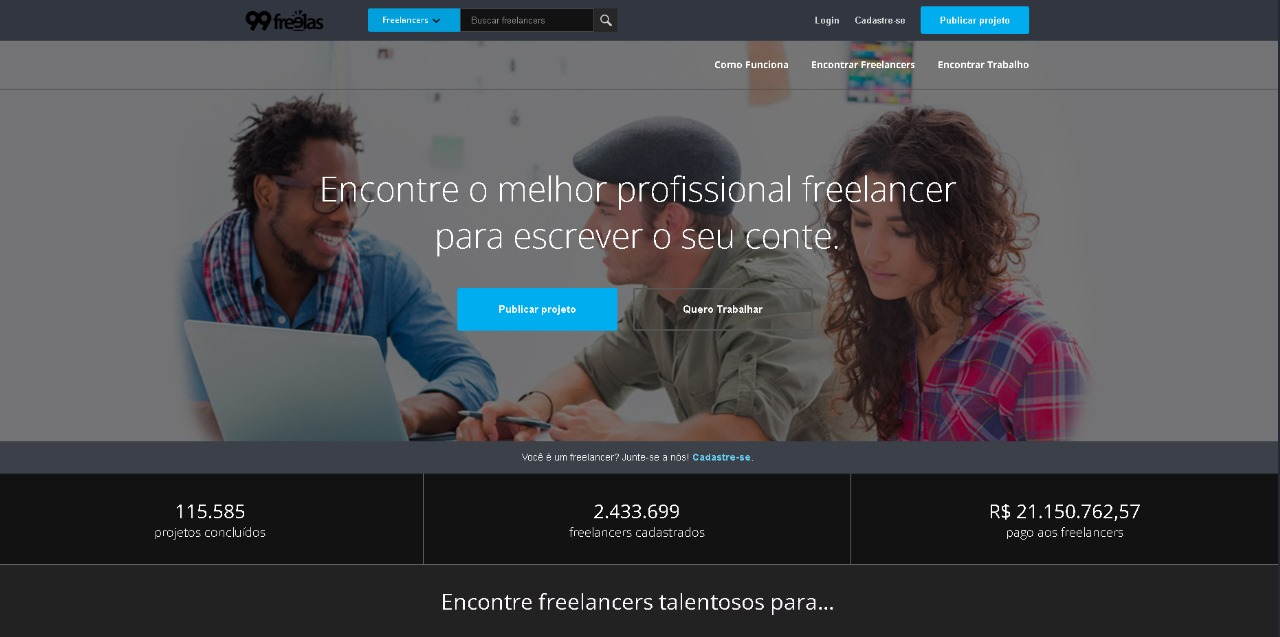
\includegraphics[scale=0.4]{Illustrations/99Freelas.jpg}
\SourceOrNote{https://www.99freelas.com.br (2024)}
\end{figure}

\section{GETNINJAS}
\subsubsection{Esta ferramenta conhecida como \cite{GetNinjas} oferece um meio de solução para contratação de serviços freelancers para diversas finalidades: serviços domésticos, saúde, moda, beleza além da compra de diversos tipos de cursos, consultorias ou até mesmo aluguel de maquinários.}

\begin{figure}[h!]
\centering
\caption{GetNinjas}
\label{fig:GetNinjas}
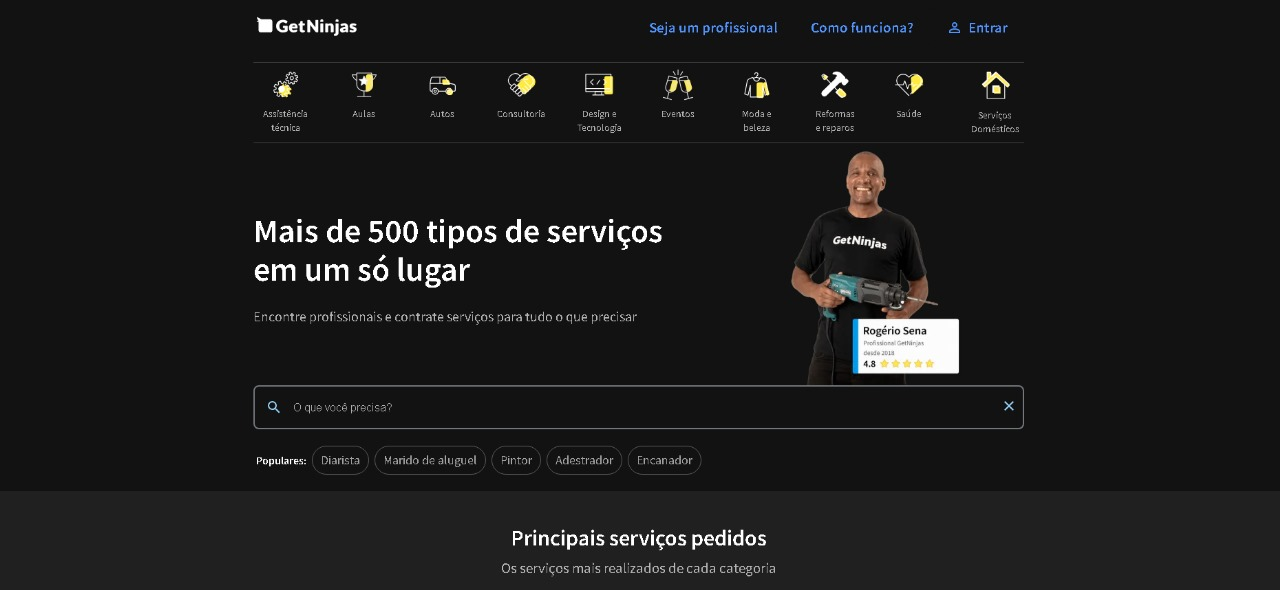
\includegraphics[scale=0.4]{Illustrations/GetNinjas.jpg}
\SourceOrNote{https://www.getninjas.com.br (2024)}
\end{figure}

\section{FIVERR}
\subsubsection{O \cite{Fiverr} é uma plataforma para intermediação de serviços relacionados a diversas áreas, como design gráfico, redação, marketing digital e programação permitindo que freelancers publiquem suas ofertas. A Fiverr conta com um sistema de avaliação que ajuda os usuários a escolher prestadores de serviços com base na reputação e na qualidade do trabalho, a plataforma também facilita a negociação e entrega de serviços, promovendo eficiência e transparência nas transações.}

\clearpage

\begin{figure}[h!]
\centering
\caption{Fiverr}
\label{fig:Fiverr}
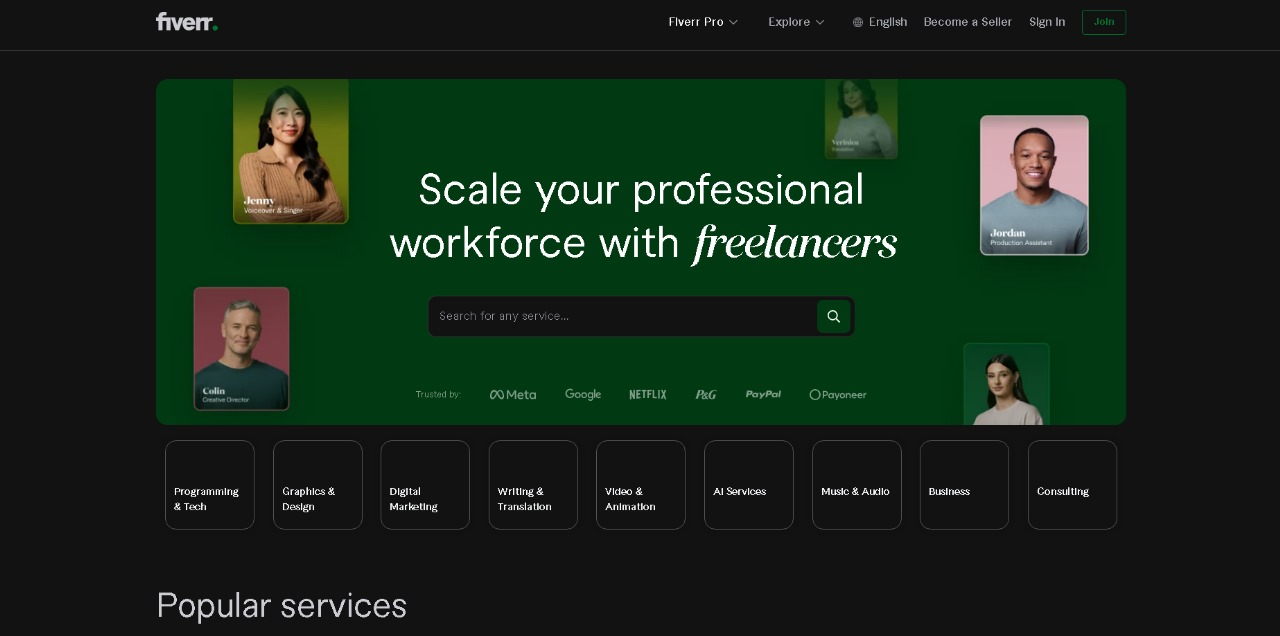
\includegraphics[scale=0.4]{Illustrations/Fiverr.jpg}
% \SourceOrNote{https://www.fiverr.com/?source=top_nav (2024)} % O vscode não tá aceitando adicionar essa fonte aqui
\end{figure}

\section{API PARA CONTRATAÇÃO DE SERVIÇOS DE INFORMÁTICA}
\subsubsection{Este estudo \cite{Silva2022} trata-se sobre uma aplicação para contratação de serviços de informática, com o intuito de ajudar iniciantes da área, por conta do tempo de experiência exigido pelos contratantes, é um auxilio para alavancar profissionais que estão ingressando no ramo tecnológico.}

\section{UTILIZAÇÃO DE API PARA GEOLOCALIZAÇÃO EM TEMPO REAL DE ENCOMENDAS PEDIDAS POR MEIO DE UM APLICATIVO MOBILE MULTIPLATAFORMA}
\subsubsection{Este projeto \cite{Oliveira2022} é uma proposta de e-commerce com serviço de geolocalização para publicação, seleção, envio e rastreio de encomendas que conecta motoristas, remetentes e destinatários para maior facilidade e agilidade da entrega.}

\begin{figure}[h!]
\centering
\caption{Utilização de api para geolocalização em tempo real de encomendas pedidas por meio de um aplicativo mobile multiplataforma}
\label{fig:Oliveira12022}
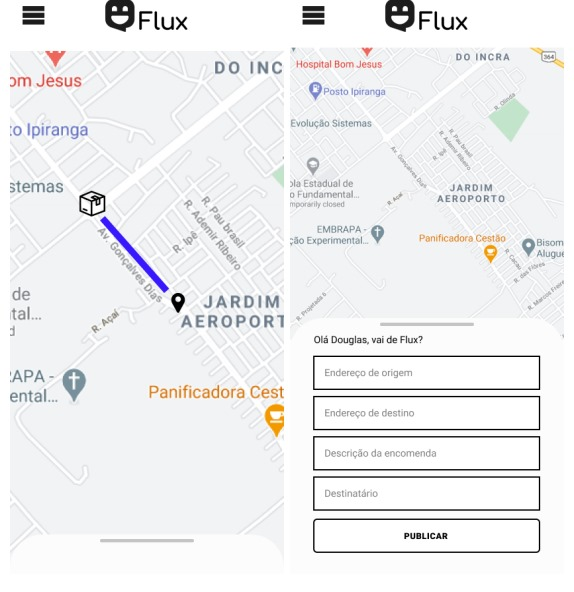
\includegraphics[scale=0.6]{Illustrations/Oliveira12002.jpg}
\SourceOrNote{https://repositorio.utfpr.edu.br/jspui/handle/1/32355(2024)}
\end{figure}